\chapter{State of the Art}
\label{lab:sota}
As already mentioned in section \ref{sec:terms}, \textit{Development}, developing software is greatly facilitated using existing building blocks instead of writing the entirety of program code from scratch. Especially Web server applications benefit from \textit{frameworks} -- i.e. third-party software that can be extended with application-specific code -- because frameworks generally provide support for standard, repetitive procedures like handling network communication, database access, caching\footnote{The \textit{cache} is mainly short-lived memory used for faster delivery of dynamic data.} and URL mapping\footnote{URL mapping is the process of deciding which action should be taken based on the requested network URL.}. The process of minimising repetitive code and maximising code reusability can be described as reducing \textit{boilerplate code} or by the acronym \textit{DRY}\footnote{Don't repeat yourself} \cite[p. 149]{Scala} \cite[p. 1]{Orsini2008}.

Modern Web frameworks often include ways of abstracting concurrency or build on existing concurrency frameworks themselves. This can save the developer from having to deal with low-level concerns like thread scheduling and message passing (see section \ref{sec:threads} and \ref{lab:actormodel}, respectively). \textit{Full-stack} Web frameworks often handle many -- if not all -- tasks common to specific networking applications. They may even include their own Web server to improve the handling of numerous concurrent requests. Inbound and outbound network communication represents a large share of common features. Also, served assets like websites and images play a role in certain use-cases (but do not in case of a purely API-focussed server). Storage in form of cache and data persistence is also important for most applications. However, asynchronous I/O and Event- and Actor-based interfaces are the main focus of this chapter. Figure \ref{fig:full_stack} gives a brief overview of typical full-stack framework capabilities. 

\begin{figure}
\centering\small
\setlength{\tabcolsep}{0mm}
  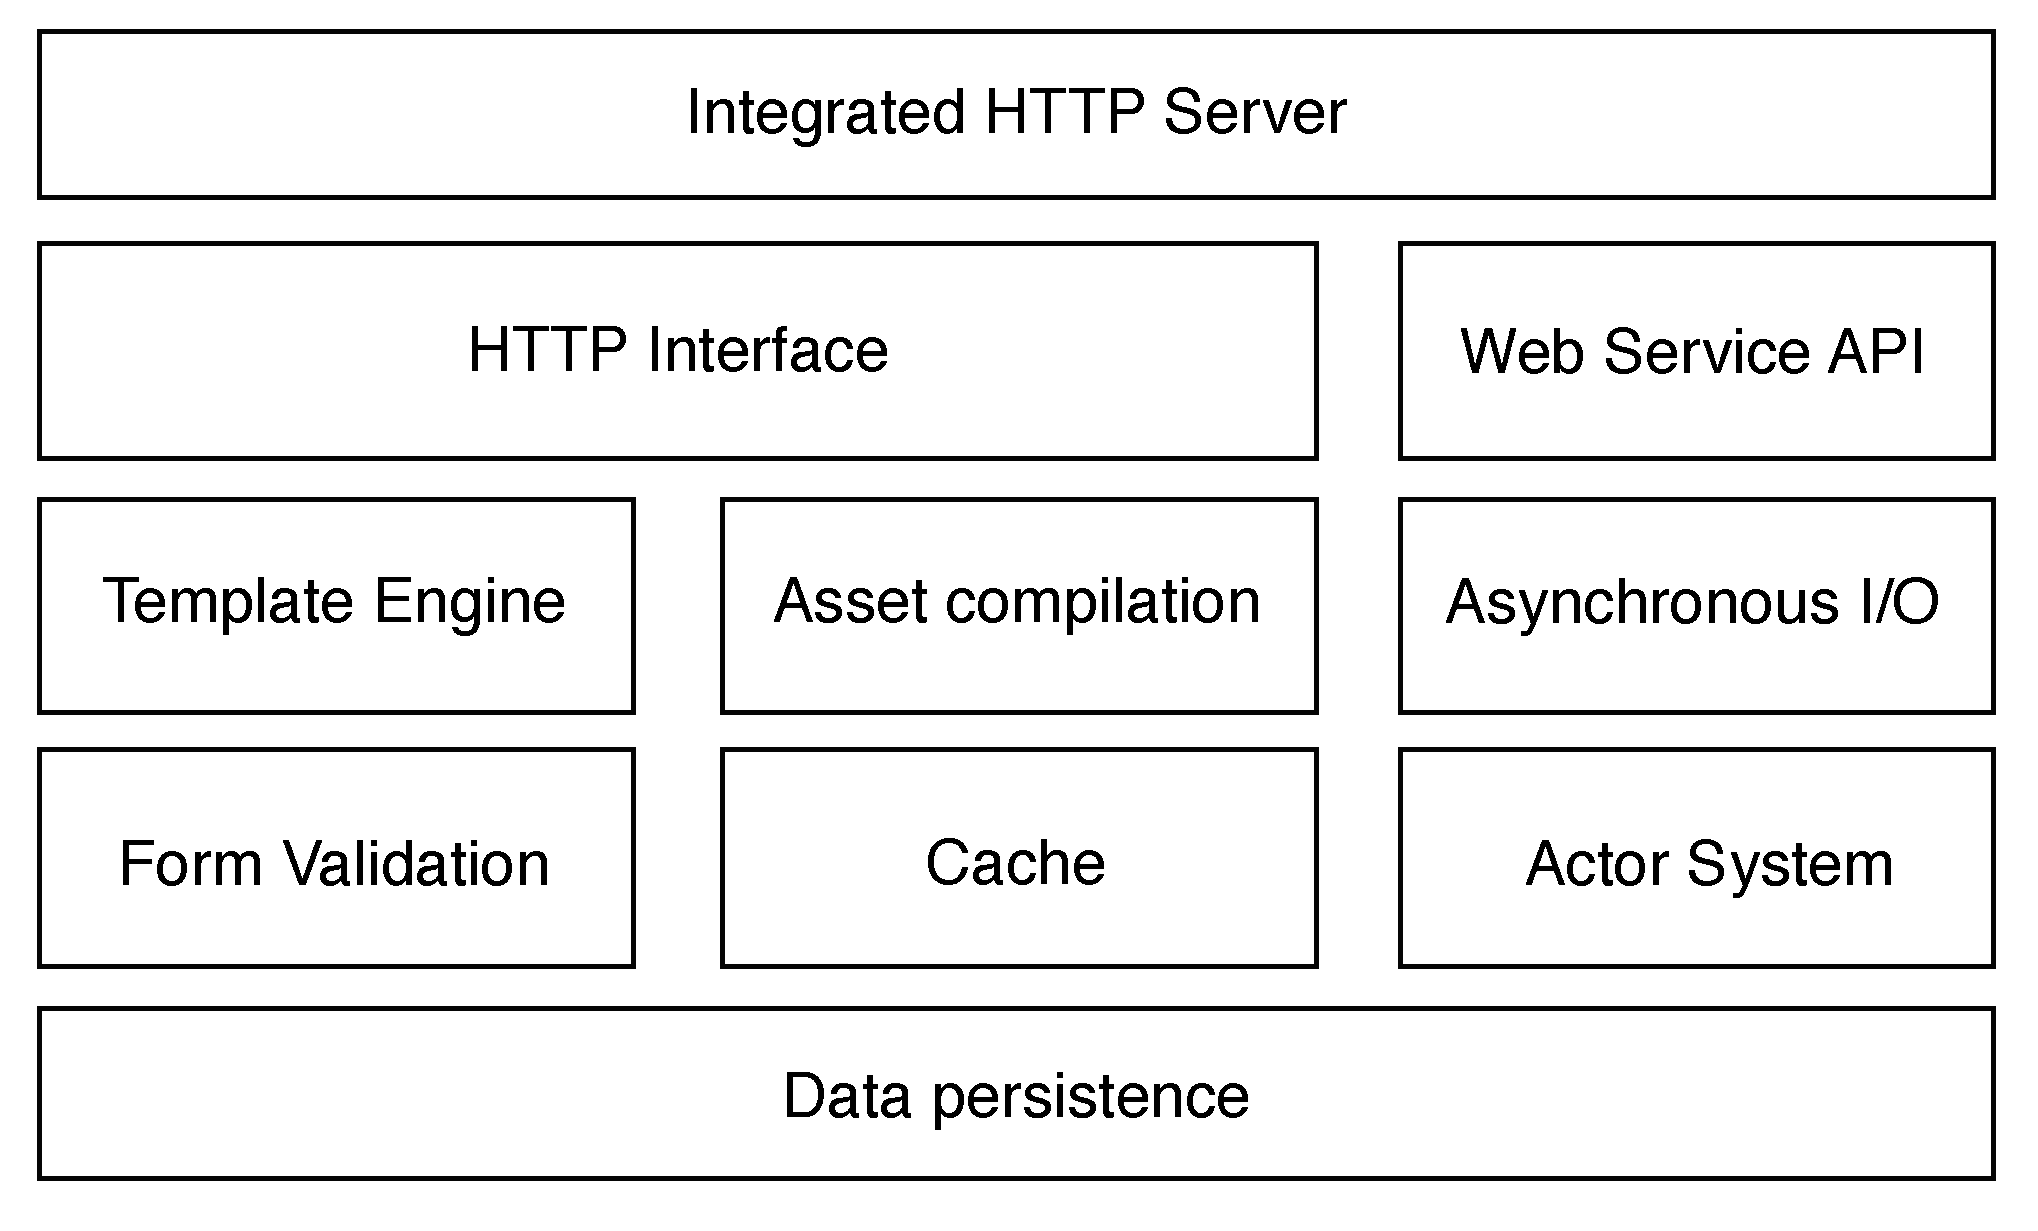
\includegraphics[width=.90\textwidth]{full_stack}
\caption{
A Web framework aims to facilitate development by including frequently used capabilities. Image based on the structure of the \textit{Play! Framework} \cite{Scala}
}
\label{fig:full_stack}
\end{figure}

This chapter presents selected approaches to performance-critical event-based and actor-based concurrency abstraction with respect to the criteria defined in section \ref{sec:terms} and taking into account the technical issues elaborated in section \ref{sec:concurrency}. The respective technologies were chosen according to their current relevancy and popularity in the current technological background and ordered with regard to their applicability in the context of this thesis.

\section{Event-based technologies}
\label{sec:evnt}

\subsection{Node.js}
\label{sec:nodejs}

\textit{Node.js}\footnote{\url{http://nodejs.org/}} is not only a framework, but rather a dedicated open source software platform for purely event-driven applications. User-level code is written in the \textit{JavaScript} scripting language and interpreted by the \textit{V8}\footnote{\url{https://code.google.com/p/v8/}} engine also used in the \textit{Google Chrome} Web browser\footnote{\url{https://www.google.com/intl/en/chrome/browser/}} \cite[p. 19]{Hughes-Croucher2012}. \textit{JavaScript} was originally used primarily for programming client-side website behaviour; however, \textit{Node.js} uses a module system\footnote{Using the \textit{CommonJS} module specification (\url{http://www.commonjs.org/})} to add various Web server-specific features. These features include -- among others -- networking abstractions, file and operating system abstractions and replication and scheduling utilities\footnote{See \url{http://nodejs.org/api/} for an exhaustive list of system modules or \url{https://www.npmjs.org/} for a popular extension module repository.}. The platform also includes its own Web server via the \texttt{http} module\footnote{\url{http://nodejs.org/api/http.html}}.

\subsubsection*{Development}
\label{lab:nodehttp}
Program modules are represented by \textit{JavaScript} files. The entry point of a program must be defined by specifying the main \textit{JavaScript} file upon application launch \cite[p. 16]{Hughes-Croucher2012}. To use a module, it can be included using the \texttt{require} command. Program flow typically propagates via callbacks (see section \ref{lab:flow}). An example of these concepts can be seen in program \ref{prog:node-http}. Due to the functional nature of \textit{JavaScript}, callback functions can be the main driving force of asynchronous program flow. The following factors support this \cite{node-loop}:
\begin{itemize}
  \item First-class functions can be handled like any other data type; they can be stored in variables, passed as parameters and executed when needed.
  \item Parts of the program flow can be composed of multiple \textit{anonymous} functions, which allows for flexible ordered execution (as seen in program \ref{prog:node-http}).
\end{itemize}
\begin{program}
  \caption{This example illustrates the concepts introduced at the beginning of section \ref{lab:nodehttp}. In line 1, a HTTP network abstraction is loaded and line 2 calls a function that requests the creation of a new server instance; this function receives an \textit{anonymous} callback function, which is called upon each incoming HTTP request. The function's two parameters are the HTTP request and response, respectively. Line 3 and 4 generate the response by setting the HTTP status code, the \texttt{Content-Type} header and the response body. The server is started via the function \texttt{listen}, which accepts a network port and IP address. Code source: \cite[p. 9]{Hughes-Croucher2012}}
  \label{prog:node-http}
  \begin{JavaCode}
var http = require('http');
http.createServer(function (req, res) {
    res.writeHead(200, {'Content-Type': 'text/plain'}); 
    res.end('Hello World\n');
}).listen(8124, "127.0.0.1");
console.log('Server running at http://127.0.0.1:8124/');
  \end{JavaCode}
\end{program}
However, there are several caveats to exclusively callback-driven program flow. For one, multiple callbacks executed sequentially are not guaranteed to return in order. There is also no predefined way of awaiting multiple callback results. Also, callbacks -- when used excessively -- tend to lead to quite unreadable code and, ultimately, to a condition known as the \textit{Pyramid of Doom} (see program \ref{prog:doom}).
\begin{program}
  \caption{Multiple dependent callback functions can lead to a structure called \textit{Pyramid of Doom}, which can impede code readability. Every step function (i.e. \texttt{step1}, \texttt{step2}, \ldots) asynchronously depends on the result of the previous one. In this example, code indentation tends to increase faster than line progression. Code source: \cite[p. 21]{Torstensson2012}}
  \label{prog:doom}
  \begin{JavaCode}
step1(function (value1) {
    step2(value1, function (value2) {
        step3(value2, function (value3) {
            step4(value3, function (value4) {
                // Do something with value4
            });
        });
    });
});	
  \end{JavaCode}
\end{program}
To relieve these problems, the \textit{promise} paradigm can be used as an abstraction for callbacks. With a promise framework like the one included in the popular \textit{jQuery} library\footnote{\url{http://jquery.com/}} or the \textit{Q} library\footnote{\url{https://github.com/kriskowal/q}}, sequential functions can be written more idiomatically as a chain of commands (see program \ref{prog:promises}). When a promise is created, the result is \textit{deferred}, i.e. returned at a later point in time. If the action of the promise was successful, the promise is \textit{resolved}, otherwise it is \textit{rejected}. There is also a comprehension (i.e. a specialised syntactic construct) that allows for resolving multiple promises in parallel and treating the results as a single array of values as soon as all promises are resolved:

\begin{JavaCode}
Q.all([stepA, stepB]).then(function (results) {
    var resultA = results[0];
    var resultB = results[1];
});
\end{JavaCode}

\begin{program}
  \caption{By using a promise library, sequential asynchronous processing can be simplified. The \texttt{then} function accepts a first-class callback function and, optionally, an error handler (as seen in line 7). Code source: \cite[p. 21]{Torstensson2012}}
  \label{prog:promises}
  \begin{JavaCode}
step1()
.then(step2)
.then(step3)
.then(step4)
.then(function (value4) {
    // Do something with value4
}, function (error) {
    // Handle any error from step1 through step4
})
  \end{JavaCode}
\end{program}

Another means of program flow in \textit{JavaScript} is via explicit events. In \textit{Node.js}, this can be conveniently done by using the \texttt{events} module\footnote{\url{http://nodejs.org/api/events.html}}. New events are created and handled by an instance of \texttt{EventEmitter} (see program \ref{prog:emitter}). This way, a very flexible (yet \textit{flat}, see section \ref{lab:flow}) program flow can be realised.

\begin{program}
  \caption{A simple example of explicit events. First, the emitter created through the \texttt{events} module registers a behaviour (in form of a callback function) for a certain event type (i.e. \texttt{doorOpen}). At an arbitrary point in time an event of this type is created and triggers the callback function. Code source: \cite{Cogneau2013}}
  \label{prog:emitter}
  \begin{JavaCode}
var events = require('events');
var eventEmitter = new events.EventEmitter();
 
var ringBell = function ringBell()
{
    console.log('ring ring ring');
}
eventEmitter.on('doorOpen', ringBell);
 
eventEmitter.emit('doorOpen');
  \end{JavaCode}
\end{program}

The \texttt{async}\footnote{\url{https://github.com/caolan/async}} module provides a number of functions that abstract and simplify working with asynchronous actions in a functional way and has an even wider scope than the \textit{Q} library. For instance, it introduces comprehensions to apply an asynchronous function to multiple values (\texttt{each()}) and facilitates control flow with helpers for serial and parallel execution:

\begin{JavaCode}
async.parallel([
    function(){ ... },
    function(){ ... }
], callback);
\end{JavaCode}

Independently of the exact method of implementing concurrency in \textit{Node.js}, \textit{inversion of control} (see section \ref{lab:events}) plays a big role and its drawbacks (e.g. reduced code readability) are hard to avoid without using special libraries \cite[p. 93]{Erb2012}. However, because \textit{JavaScript} is a very popular language due to its use in website development, the fast adoption rate and shallow learning curve of \textit{Node.js} help with building a rich ecosystem around the platform \cite[p. 27]{Hughes-Croucher2012}.

\textit{Node.js} applications can also benefit from certain framework modules that add \textit{MVC}\footnote{Model-View-Controller} capabilities. One such module is the \textit{express} framework\footnote{\url{http://expressjs.com/}}, which includes features such as advanced routing and templates and brings \textit{Node.js} one step closer to being a full-stack Web framework.

\subsubsection*{Scalability}
Applications running on \textit{Node.js} per default only use a single thread for processing \cite{node-loop}. As mentioned in the previous chapter, this has a positive effect on scheduling overhead. Because of the nature of \textit{JavaScript} and \textit{Node.js} (e.g. asynchronous networking and file abstractions as well as the use of callbacks), it is comparably easy to write code that does not block the processing thread. However, \textit{if} blocking occurs, the consequence is that the whole application is unable to process any requests until the blocking action has finished. On the other hand, this removes any need for synchronisation concerns and prevents address space conflicts between threads \cite[p. 105]{Erb2012}.

To scale out (see section \ref{lab:scalabilty}) a \textit{Node.js}-based application, two main steps can be taken: Scaling out only on a single multi-core machine or scaling out on multiple machines. The first can be archived by creating multiple instances of the same program using the \texttt{cluster} module\footnote{\url{http://nodejs.org/api/cluster.html}} of \textit{Node.js} (see program \ref{prog:cluster}). This way, a master process obtains control over several child processes that handle requests asynchronously based on load balancing \cite[p. 64]{Hughes-Croucher2012}. The technique of having one process create child instances is called forking. If forking is not supported by the operating system (e.g. on \textit{Windows}\footnote{http://windows.microsoft.com/} systems), the application creates multiple threads in the same process. Running the application on multiple servers has no special implications for \textit{Node.js}; if shared state is desired, it has to be archived by a messaging protocol like \textit{pub-sub} \cite[p. 137]{Hughes-Croucher2012}.

\begin{program}
  \caption{The \texttt{cluster} module provides an abstraction of creating multiple instances of a program. The first process executing the code is defined as the master process and all other processes (the number of processes depends on the number of processing cores in the system) are forked as child processes. Code source: \cite{Hughes-Croucher2012}}
  \label{prog:cluster}
  \begin{JavaCode}
var cluster = require('cluster'); 
var http = require('http');
var numCPUs = require('os').cpus().length;

if (cluster.isMaster) {
    // Fork workers.
    for (var i = 0; i < numCPUs; i++) {
        cluster.fork();
    }
    ...
} else {
    // Worker processes have a http server.
    http.Server(function(req, res) {
        res.writeHead(200);
        res.end("hello world\n");
    }).listen(8000);
}
  \end{JavaCode}
\end{program}

\subsubsection*{Performance}
\textit{Node.js} is considered very suitable for massive connection concurrency and data-heavy applications \cite[p. 44]{Torstensson2012}. The \textit{V8} engine executes \textit{JavaScript} code at a very favourable speed; interfaces that often slow down browser-based applications (like the \textit{DOM}\footnote{Document Object Model}) are not present in a server-side environment. However, since the code is executed via interpretation, its execution is inherently slower than the execution of binary files or virtual machine bytecode. Figure \ref{fig:node_performance} illustrates the serious implications of intensive computations on response time. 

\begin{figure}
\centering\small
\setlength{\tabcolsep}{0mm}
  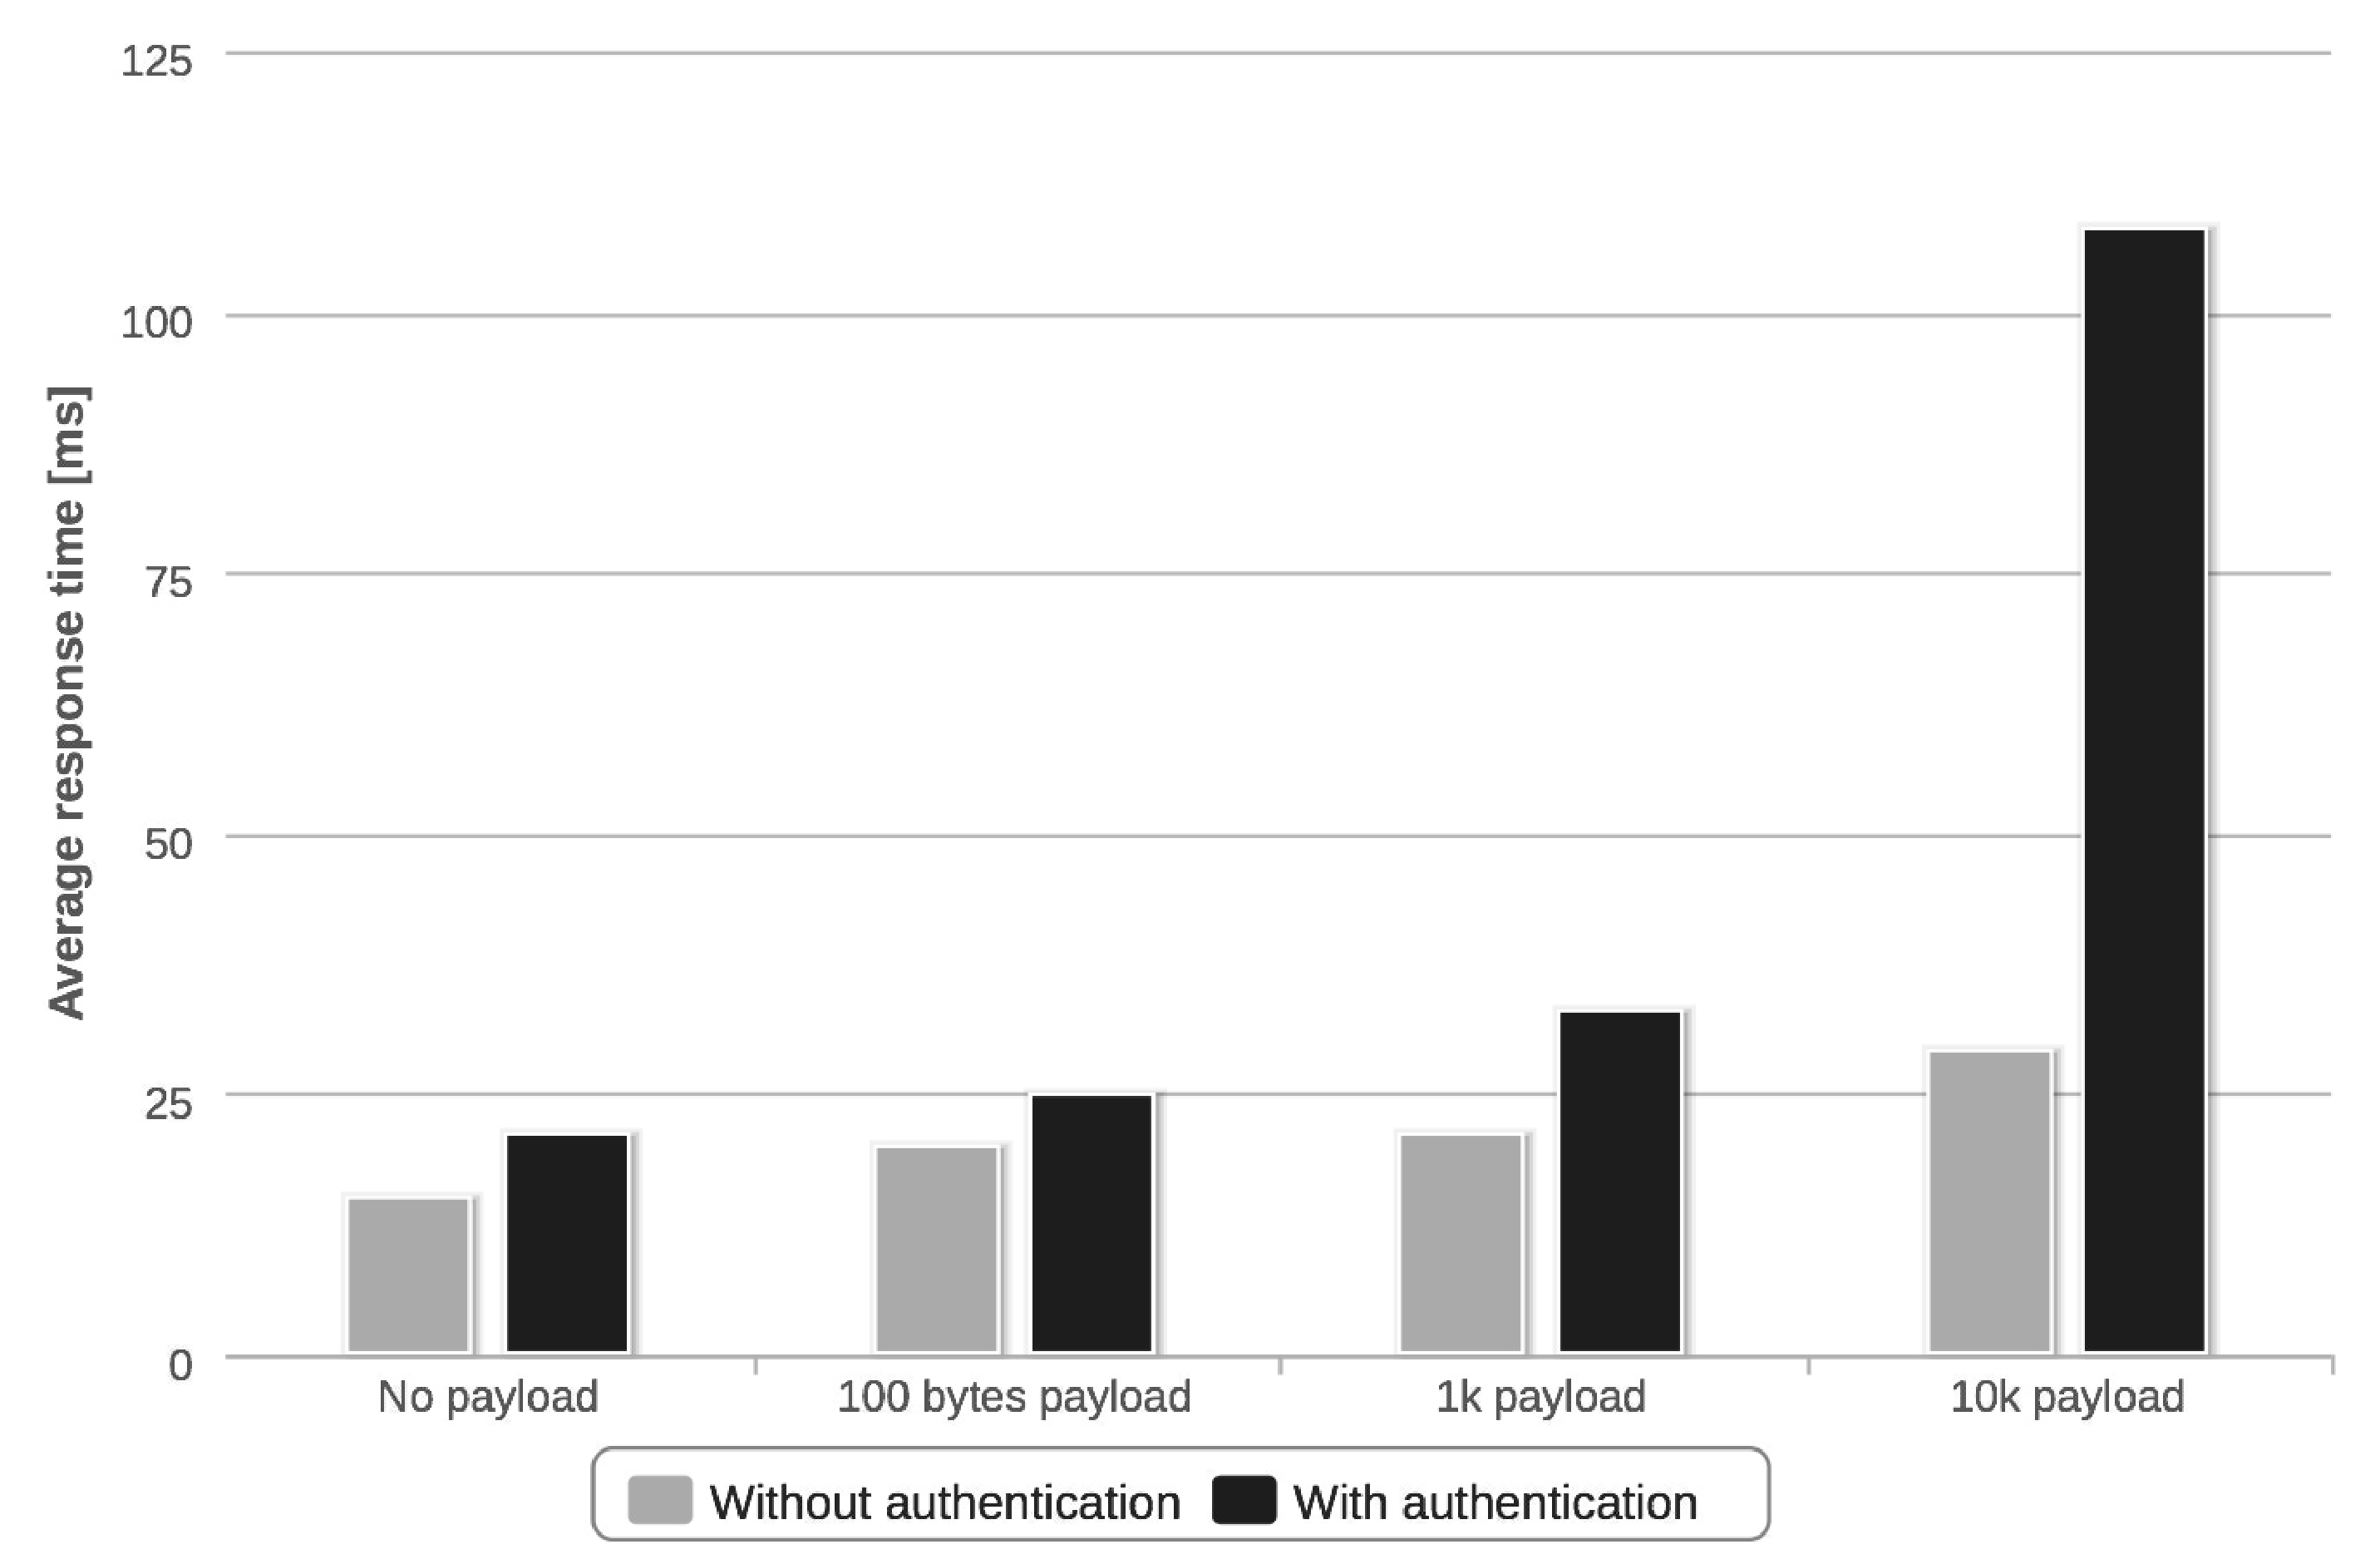
\includegraphics[width=.80\textwidth]{node_performance}
\caption{
In this figure taken from a performance analysis of D. Torstensson and E. Eloff, requests are sent to a \textit{Node.js} server with different payload sizes. The requests are sent both with and without authentication; authentication is done by hashing (i.e. processing) the whole payload using the \textit{SHA1-HMAC} algorithm. Larger payloads are more computationally intensive and result in a longer response time. Image source: \cite{Torstensson2012}.
}
\label{fig:node_performance}
\end{figure}

\subsection{Eventmachine}
\label{sec:eventmachine}
Ruby\footnote{\url{https://www.ruby-lang.org}} is a dynamic programming language that has a high adoption rate due to the popular \textit{Ruby on Rails} MVC framework that powers a lot of modern Websites \cite[p. 11]{Orsini2008}. However, unlike \textit{JavaScript}, \textit{Ruby} was not conceived with non-blocking event-driven behaviour in mind. \textit{Eventmachine}\footnote{\url{http://rubyeventmachine.com/}} is a library that aims to facilitate the process of developing non-blocking Web server applications in \textit{Ruby}.

\subsubsection*{Development}
As mentioned in section \ref{lab:nodehttp}, \textit{JavaScript} uses anonymous and first-order functions to manage asynchronous program flow. Due to \textit{Ruby's} object-oriented nature, these concepts are not supported at language-level; instead, it supports so-called \textit{blocks} that in some way can act like anonymous functions and receive parameters from previous operations \cite{Fitzgerald2007}. See program \ref{prog:ruby-sync} for a simple demonstration of how blocks can be used to create a basic networking server.

\begin{program}
  \caption{This program demonstrates how blocks can be used with the \texttt{TCPServer} library (included in \textit{Ruby's} standard library) to create a new thread for every incoming network client. The block (line 4 to 8) acts as a container applied to the result of previous operations, similar to a closure in \textit{JavaScript}; the \texttt{client} variable is the result of the \texttt{new} method of the \texttt{Thread} class, which accepts a \texttt{TCPSocket} object. Code source: \cite {Gupta2010}}
  \label{prog:ruby-sync}
  \begin{JavaCode}
require 'socket'
server = TCPServer.new(2202)
while true
    Thread new(server.accept){ |client|
        msg = client.readline
        client.write "You said: #{msg}"
        client.close
    }
end
  \end{JavaCode}
\end{program}

To create a non-blocking networking server in \textit{Ruby}, more complex operations are needed. This includes creating and managing a complete event-loop\footnote{Strictly speaking, since no events are involved, this is called a \textit{reactor loop} \cite{Gupta2010}.} and using the \texttt{IO} class and the \texttt{accept\_nonblock} method of the \texttt{TCPSocket} class to create logical concurrency on one thread (an exhaustive example can be seen in \cite{Gupta2010}). Operations like handling connections and reading input from the sockets also have to be managed explicitly by the developer \cite{Gupta2010}.

\begin{program}
  \caption{A simple echo server, i.e. a server that responds in a simple way depending on what the request contains. A \textit{Ruby} module (line 5) contains the necessary logic and is managed by the \textit{EventMachine} system. Line 10 initialises the reactor loop and line 11 starts the server using the predefined module.}
  \label{prog:ruby-em}
  \begin{JavaCode}
require 'rubygems'
require 'eventmachine'

module EchoServer
    def receive_data data
        send_data "You said: #{data}"
    end
end

EventMachine::run {
    EventMachine::start_server "127.0.0.1", 2202, EchoServer
}
  \end{JavaCode}
\end{program}

\textit{EventMachine} provides a simple way to abstract the process of managing event-based concurrency with \textit{Ruby}. It includes its own event-loop -- or \textit{reactor} -- which creates and handles events across the application. To interact with the environment, the reactor provides asynchronous interfaces -- called \textit{Connections}, which have to be defined within the reactor loop. \textit{EventMachine} includes several ways of creating connections:

\begin{itemize}
  \item Creating a subclass of the \texttt{Connection} class and overriding its methods, then passing the class reference to the \textit{connect} method of \textit{EventMachine}
  \item Creating a module with the appropriate methods for handling connections (see program \ref{prog:ruby-em})
  \item Using a block (see program \ref{prog:ruby-sync}) and overriding methods of the connection object passed as parameter
\end{itemize}
Program \ref{prog:ruby-em} demonstrates, how the simple TCP server from program \ref{prog:ruby-sync} can be implemented using the \textit{EventMachine} reactor. Besides this comprehensible TCP communication functionality, \textit{EventMachine} also includes functionality for deferring or postponing program logic. Deferring is important when interacting with code that would normally block the event-loop (see program \ref{prog:ruby-defer}). The \texttt{Timer} class or the \texttt{add\_timer} and \texttt{add\_periodic\_timer} methods can be used to execute program logic at an arbitrary point in time (e.g. for scheduled or recurring tasks). There is also a \texttt{Queue} comprehension for managing multiple asynchronous tasks at once (cf. the \texttt{all} comprehension of the \textit{Q} library in section \ref{lab:nodehttp}). 

\begin{program}
  \caption{An example of using \textit{EventMachine} to achieve \textit{JavaScript}-like callback functionality in \textit{Ruby}. A long-running operation can be put in a block, the execution of which is managed by \textit{EventMachine} via its threadpool. After the execution has completed, the result is passed to another block (i.e. the ``callback'') as a parameter.}
  \label{prog:ruby-defer}
  \begin{JavaCode}
operation = proc {
    # long-running operation, e.g. database query
}
callback = proc { |result|
    # do something with result
}

EventMachine.defer(operation, callback)
  \end{JavaCode}
\end{program}

\subsubsection*{Scalability and Performance}
Like \textit{JavaScript}, \textit{Ruby} is an interpreted scripting language and as such performance is inherently inferior to compiled languages\footnote{However, Web servers that focus heavily on I/O-bound operations like network and database communication may not need as much CPU performance as e.g. a server used for image processing.} (cp. section \ref{sec:nodejs}, \textit{Performance}). When using the default \textit{Ruby} VM\footnote{Virtual Machine, a program that executes code inside a dedicated environment.}, a security measure called \textit{Global Interpreter Lock} prevents program threads from archiving physical concurrency by only executing one logical thread at once (see figure \ref{fig:gil}). This is done to prevent sharing non thread-safe code with other threads \cite{ruby-gil}. Thus, to scale a \textit{Ruby} application running on the default virtual machine, several process instances have to be created. This is similar to \textit{Node.js} and many implications that apply to scaling \textit{Node.js} applications also apply to \textit{Ruby}. \textit{JRuby}\footnote{\url{http://jruby.org/}} is an alternative implementation of the standard \textit{Ruby} interpreter which theoretically allows for controlling physical concurrency at application level \cite{ruby-gil}.

\begin{figure}
\centering\small
\setlength{\tabcolsep}{0mm}
  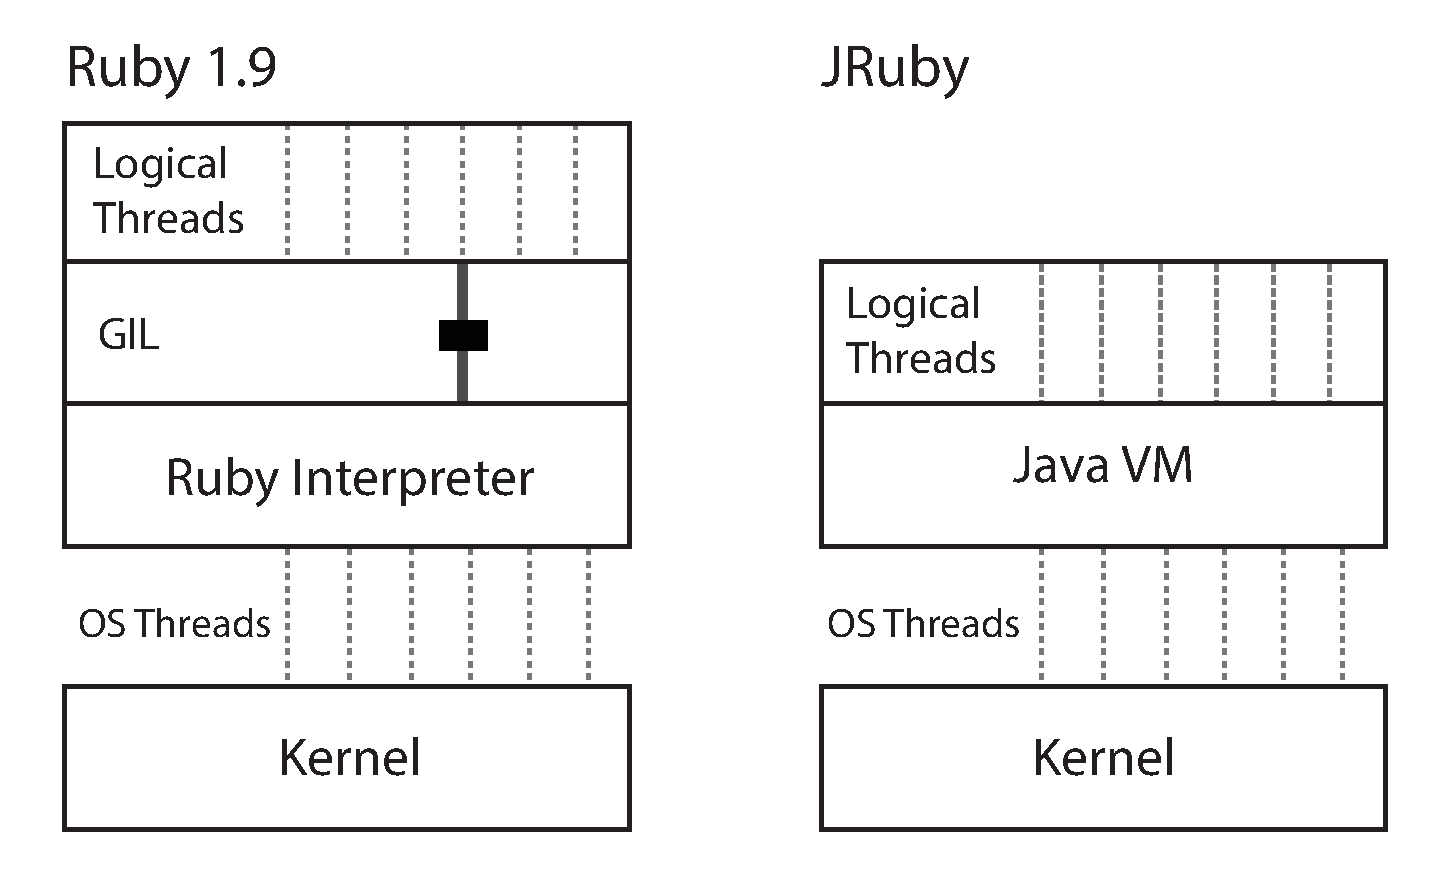
\includegraphics[width=.80\textwidth]{ruby-gil}
\caption{
The \textit{Global Interpreter Lock} of the \textit{Ruby} VM prevents application logic to control parallel program execution on OS threads because it executes only one \textit{Ruby} thread at once. However, with \textit{JRuby}, this is possible. Image source: \cite{ruby-gil}.}
\label{fig:gil}
\end{figure}

\subsection{Others}
\label{lab:other-event}
There are numerous other examples of event-driven concurrency frameworks that are less documented or fitting to be presented in depth here. \textit{React}\footnote{\url{http://reactphp.org/}} is a framework written in \textit{PHP}\footnote{\url{https://php.net/}}, a scripting language that is often used in simple Web server applications \cite[p. 36]{Erb2012}. \textit{Twisted}\footnote{\url{https://twistedmatrix.com/}} is a reactor library for the \textit{Python}\footnote{\url{https://www.python.org/}} scripting language; its capabilities are similar to the \textit{EventMachine} library presented in section \ref{sec:eventmachine}. \textit{Java NIO}\footnote{Native Input and Output} (see section \ref{lab:flow}) is a general interface for non-blocking I/O operations that allows for creating asynchronous Web server applications on a low level.

\section{Actor-based technologies}

\subsection{Play!}
\label{lab:play}
\textit{Play!}\footnote{\url{http://www.playframework.com/}} is a full-stack Web application framework for development in \textit{Scala}\footnote{\url{http://www.scala-lang.org/}} and \textit{Java}. Since both languages are compiled to \textit{Java} bytecode and run on the \textit{Java} VM, both languages can be used side by side and libraries from the exhaustive \textit{Java} ecosystem can be included; as of version 2, the \textit{Play!} framework is written solely in \textit{Scala} \cite{Scala}. \textit{Play!} uses the \textit{Akka}\footnote{\url{http://akka.io/}} actor system, which is -- like the \textit{Scala} language and \textit{Play!} itself -- managed by \textit{Typesafe Inc.}\footnote{\url{https://typesafe.com/}}; all three products are available as an integrated environment called \textit{Activator}. 

\subsubsection*{Development}
\textit{Play!} is different from all aforementioned frameworks (see section \ref{sec:evnt}), not only in the sense that it uses actor-based concurrency, but also in that it is based on a compiled programming language rather than an interpreted scripting language. Existing since 2003, \textit{Scala} is a rather young programming language that is syntactically very similar to \textit{Java}, but extends it with functional programming capabilities and a more sophisticated type system. Since it has native support for comprehensions associated with concurrency and a more concise syntax, it is better suited for applications with a high amount of application-level concurrency operations \cite[p. 9]{Scala}; therefore, in this section \textit{Play!}'s functionality is presented using \textit{Scala}.

\textit{Play!} builds upon the MVC model, which means that incoming requests are handled by a user-defined controller structure. A controller contains \textit{Actions}, i.e. methods that mapped to certain types of requests. Each controller method must return an object of the class \texttt{Result}, which contains the data to be sent back to the client \cite[p. 27]{Reelsen2011}. When defining an action, there are two basic types of actions in terms of concurrency -- synchronous and asynchronous. Asynchronous actions must return an object of the type \texttt{Future[Result]}. A \textit{future} is similar to a \textit{promise} (see section \ref{sec:nodejs}, \textit{Development}) and indicates that the result is not available at the momentary point of execution, but at an arbitrary time in the future; only when the calculation of the result has finished (either successfully or due to failure) the response is sent to the client (see program \ref{prog:scala-actions1} and \ref{prog:scala-actions2}, respectively) \cite[p. 86]{Scala}. 

\begin{program}
  \caption{This program contains a very simple demonstration of how application-level code integrates with the \textit{Play!} framework. \texttt{def} defines a new method, which is wrapped by the \texttt{Action} constructor method. The actual method logic is passed to the \texttt{Action} wrapper as a block, which has to return a \texttt{Result} object. The \texttt{Ok} method in line 4 converts a string to a \texttt{Result} object with the HTTP status code 200, indicating a successful operation with a non-empty response.}
  \label{prog:scala-actions1}
  \begin{JavaCode}
// Synchronous action
def shortProcessingRequest = Action {
    val result = (2 + 2).toString
    Ok(result)
}
  \end{JavaCode}
\end{program}
\begin{program}
  \caption{Returning asynchronous results is slightly more complex than returning synchronous results (see program \ref{prog:scala-actions1}). Using the \texttt{async} method of the \texttt{Action} object, a block returning a future result can be invoked. The \texttt{ContactDatabase.findById} method is a fictional database query that returns e.g. a \texttt{Future[Contact]} object. Since the block expects a \texttt{Future[Result]} object as a return value, the database result has to be \textit{mapped} to an action result. The \texttt{map} method invokes a new block, which is executed when the future operation is resolved successfully. This block receives the non-future result as a parameter, which is wrapped by the \texttt{Ok} method. Thus, the result type of the statement in line 3 changes from \texttt{Future[Contact]} to \texttt{Future[Result]}.}
  \label{prog:scala-actions2}
  \begin{JavaCode}
// Asynchronous action
def longDatabaseRequest = Action.async {
    ContactDatabase.findById(123) map {
        result =>
            Ok(result.toString)
    }
}
  \end{JavaCode}
\end{program}

\textit{Scala} provides various language features and libraries for handling concurrency like the \texttt{scala.concurrent} library, which includes versatile comprehensions for resolving one or multiple future results. However, \textit{Play!} includes the \textit{Akka} actor system and the respective libraries to even further facilitate concurrent processing. \textit{Akka} is used by \textit{Play!} internally for various tasks like request handling, but it can also be used at application-level \cite[p. 83]{Scala}. The actor system can be used for scheduling one-time and recurring operations, but its eponymous use is to manage actors (see section \ref{lab:actormodel}). In \textit{Play!}, explicitly used actors are well-suited for autonomous tasks like handling communication with third-party Web services or sending emails. Program \ref{prog:scala-actors} demonstrates a simple actor used to send emails. The actor class inherits from the \texttt{Actor} class of the \textit{Akka} library. As mentioned in section \ref{lab:actormodel}, actors do not share any state and communicate via messages. The actor class has to implement the \texttt{receive} method, which is called when messages arrive. Messages can have any type, but are usually sent via different \textit{case classes}, depending on the context of the message. For sending an email, these classes would contain for instance an email address and some text content. The \texttt{receive} method uses a block with \textit{pattern matching} to determine the message type. Based on the message type, different actions can be taken by the actor. To send a message to an actor, the actor reference can be generated by the actor system. Messages can be sent using the \texttt{!} method, the \texttt{?} method can be used to ``ask'' the actor, i.e. send a message and act upon a future response.

\begin{program}
  \caption{This program is a demonstration of a simple actor used to send emails.}
  \label{prog:scala-actors}
  \begin{JavaCode}
case class DefaultMail(
    email: String,
    content: String
)

case class ImageMail(
    email: String,
    image: String
)

class Mailer extends Actor {
    
    def receive = {
        case DefaultMail(email, content) =>
            sendDefaultMail(email, content)
        case ImageMail(email, image) =>
            sendImageMail(email, image)
    }

    def sendDefaultMail ...

    def sendImageMail ...

}

class Test {
    
    val mailer = Akka.system.actorOf(Props[Mailer])

    def test() = {
        mailer ! DefaultMail("john@doe.com", "Hello John")
    }

}
  \end{JavaCode}
\end{program}

\subsubsection*{Scalability}
Scala -- even though its name being a portmanteau of the words \textit{scalable} and \textit{language} -- does not support scalable actor systems at language level. It only makes assumptions about the underlying host's thread model \cite[p. 3]{Haller2009}. The majority of \textit{Play!}'s scalability is due to the included \textit{Akka} actor system \cite[p. 16]{Gupta2012}. How exactly this system behaves depends on the runtime configuration, which is defined via configuration files. Actors are generally associated with a certain \textit{execution context}, i.e. a certain configuration of the actor system. In \textit{Akka}, there are two main types of execution contexts or \textit{executors}:

\begin{description}
  \item[Thread pool executor] Multiple worker threads are preallocated and incoming messages are distributed among free threads -- this minimises thread overhead
  \item[Fork join executor] If the amount of work for single messages exceeds a certain size, the task can be split among multiple processing cores by creating (i.e. \textit{forking}) multiple instances of tasks that distribute work among them
\end{description}

Each execution context allows for configuring the minimum and maximum number of threads that are used as well as a multiplication factor that is based on the available cores. This allows for a very specific configuration of the actor system: If an execution context tends to dispatch many small tasks, the maximum number of threads can be increased, if there are few large tasks, fewer threads should be used \cite[p. 105]{Gupta2012}.

There is also a number of different dispatcher types to choose from, depending on whether actors should share a mailbox and the order in which actors are handled. Furthermore, the behaviour of mailboxes upon exhaustion can also vary from neglecting new messages to not being sent new messages \cite[p. 104]{Gupta2012}. 

All these configuration options account to the single-system scalability of \textit{Akka}. However, actors are not bound to reside on one single system. The means of communication between actors is not specified and can also be done using networking with remote systems. The default implementation of communication between different \textit{Akka} systems uses TCP and the \texttt{akka://} URL scheme. The orchestration of the entirety of actor subsystems is done by a master node system that handles message dispatching \cite[p. 233]{Gupta2012}. This way, \textit{Akka} can be scaled out to a large number of systems.

\subsubsection*{Performance}
\textit{Play!} internally uses the \textit{Netty}\footnote{\url{http://netty.io/}} HTTP server, which builds upon \textit{Java NIO} (see section \ref{lab:other-event}) to achieve non-blocking I/O capabilities \cite[p. 52]{Scala}. While \textit{Netty} has proven to be capable of serving more than 40000 requests per second\footnote{Tested on an \textit{Amazon EC2} cluster (\url{http://aws.amazon.com/ec2/})}, this on only pure network communication without Web-specific processing and I/O involved. The same request-based tests conducted on a \textit{Play!} application yield 9000 requests per second. Even with website-typical database operations and processing, a single \textit{Play!} application can serve 1350 to 2400 request per second \cite{Papauschek2013}. What is also noteworthy is that due to the adaptive nature of its actor system, \textit{Play!} delivers formidable performance even without the need for any application-level configuration.

\subsection{Lattice}
\textit{Lattice}\footnote{\url{https://github.com/celluloid/lattice}} is a lightweight Web framework for the \textit{Ruby} scripting language (see section \ref{sec:eventmachine}). It actually represents a combination of several different technologies that make up the entirety of the framework. \textit{Lattice} uses the \textit{Celluloid} actor system\footnote{\url{http://celluloid.io/}} for processing and builds upon the \textit{Reel}\footnote{\url{https://github.com/celluloid/reel}} Web server. On application level, it uses the \textit{Ruby} port of \textit{Webmachine}\footnote{\url{https://github.com/seancribbs/webmachine-ruby}}, which was originally written in \textit{Erlang}\footnote{\url{http://www.erlang.org/}}, to facilitate the handling of HTTP requests by mapping URL routes to respective controller methods \cite{Storimer2013}. 
 
Program \ref{prog:ruby-actors} demonstrates how to create actors with \textit{Celluloid}. By including the \texttt{Celluloid} object in a default \textit{Ruby} class body, actor functionality is added to the class. When creating an instance of this class, a new \textit{Celluloid} actor is initialised. To execute an asynchronous routine, the \texttt{async} method of the actor object has to be called, followed by the respective method name.

\begin{program}
  \caption{This program is an adaption of the actor example presented in program \ref{prog:scala-actors}. \textit{Celluloid} actors can be created by simple including the \texttt{Celluloid} object inside a \textit{Ruby} class.}
  \label{prog:ruby-actors}
  \begin{JavaCode}

class Mailer
    
    include Celluloid

    def send_default_mail(email, content)
        send_mail(...)
    end

    def send_image_mail(email, image)
	    send_mail(...)
    end

end

class Test

    mailer = Mailer.new

    def test()
    
        mailer.async.send_default_mail("john@doe.com, "Hello John")

    end   

end
  \end{JavaCode}
\end{program}

When using the \texttt{async} method on an actor (as seen in program \ref{prog:ruby-actors}), no value is returned. However, using the \texttt{future} method returns a \texttt{Celluloid::Future} object, which represents a rather primitive promise (see section \ref{lab:nodehttp}). There is also an explicit way of creating promises by creating a new instance of the \texttt{Celluloid::Future} object with a block parameter containing the asynchronous logic. The only way to resolve a promise is to block current execution and wait for completion; there are no comprehensions like mapping or resolving multiple promises at once \cite{Arcieri2012}.

\subsection{Others}
Apart from the above frameworks, there are hardly any full-stack Web frameworks that use the actor concurrency model. \textit{Lift}\footnote{\url{http://liftweb.net/}} is another example of a \textit{Scala}-based actor-driven framework that is similar to \textit{Play!}. However, there is no option to develop applications in \textit{Java}, it does not offer versatile actor functionality compared to \textit{Akka} and the ecosystem (i.e. support by other developers) is not as advanced as with \textit{Play!}. \textit{Xitrum}\footnote{\url{http://xitrum-framework.github.io/}} is another \textit{Scala}- and \textit{Akka}-based Web framework that aims to offer functionality similar to \textit{Lift}. \textit{spray}\footnote{\url{http://spray.io}} is a lightweight general-purpose I/O framework also based on \textit{Scala} and \textit{Akka}. It offers a number of modules for extension, including \textit{spray-can} and \textit{spray-http}, which can be used to implement a low-level HTTP server.




